\def\year{2019}\relax
%File: formatting-instruction.tex
\documentclass[letterpaper]{article} % DO NOT CHANGE THIS
\usepackage{aaai19}  % DO NOT CHANGE THIS
\usepackage{times}  % DO NOT CHANGE THIS
\usepackage{helvet} % DO NOT CHANGE THIS
\usepackage{courier}  % DO NOT CHANGE THIS
\usepackage[hyphens]{url}  % DO NOT CHANGE THIS
\usepackage{graphicx} % DO NOT CHANGE THIS
\urlstyle{rm} % DO NOT CHANGE THIS
\def\UrlFont{\rm}  % DO NOT CHANGE THIS
\usepackage{graphicx}  % DO NOT CHANGE THIS
\frenchspacing  % DO NOT CHANGE THIS
\setlength{\pdfpagewidth}{8.5in}  % DO NOT CHANGE THIS
\setlength{\pdfpageheight}{11in}  % DO NOT CHANGE THIS

%PDF Info Is REQUIRED.
% For /Author, add all authors within the parentheses, separated by commas. No accents or commands.
% For /Title, add Title in Mixed Case. No accents or commands. Retain the parentheses.
 \pdfinfo{
/Title (Sentiment Analysis on Amazon Fine Food Review Dataset)
/Author (Xinyi Li, Hongzhi Liu, Sheng Wang, Siyu Zhang)
} %Leave this	
% /Title ()
% Put your actual complete title (no codes, scripts, shortcuts, or LaTeX commands) within the parentheses in mixed case
% Leave the space between \Title and the beginning parenthesis alone
% /Author ()
% Put your actual complete list of authors (no codes, scripts, shortcuts, or LaTeX commands) within the parentheses in mixed case. 
% Each author should be only by a comma. If the name contains accents, remove them. If there are any LaTeX commands, 
% remove them. 

% DISALLOWED PACKAGES
% \usepackage{authblk} -- This package is specifically forbidden
% \usepackage{balance} -- This package is specifically forbidden
% \usepackage{caption} -- This package is specifically forbidden
% \usepackage{color (if used in text)
% \usepackage{CJK} -- This package is specifically forbidden
% \usepackage{float} -- This package is specifically forbidden
% \usepackage{flushend} -- This package is specifically forbidden
% \usepackage{fontenc} -- This package is specifically forbidden
% \usepackage{fullpage} -- This package is specifically forbidden
% \usepackage{geometry} -- This package is specifically forbidden
% \usepackage{grffile} -- This package is specifically forbidden
% \usepackage{hyperref} -- This package is specifically forbidden
% \usepackage{navigator} -- This package is specifically forbidden
% (or any other package that embeds links such as navigator or hyperref)
% \indentfirst} -- This package is specifically forbidden
% \layout} -- This package is specifically forbidden
% \multicol} -- This package is specifically forbidden
% \nameref} -- This package is specifically forbidden
% \natbib} -- This package is specifically forbidden -- use the following workaround:
% \usepackage{savetrees} -- This package is specifically forbidden
% \usepackage{setspace} -- This package is specifically forbidden
% \usepackage{stfloats} -- This package is specifically forbidden
% \usepackage{tabu} -- This package is specifically forbidden
% \usepackage{titlesec} -- This package is specifically forbidden
% \usepackage{tocbibind} -- This package is specifically forbidden
% \usepackage{ulem} -- This package is specifically forbidden
% \usepackage{wrapfig} -- This package is specifically forbidden
% DISALLOWED COMMANDS
% \nocopyright -- Your paper will not be published if you use this command
% \addtolength -- This command may not be used
% \balance -- This command may not be used
% \baselinestretch -- Your paper will not be published if you use this command
% \clearpage -- No page breaks of any kind may be used for the final version of your paper
% \columnsep -- This command may not be used
% \newpage -- No page breaks of any kind may be used for the final version of your paper
% \pagebreak -- No page breaks of any kind may be used for the final version of your paperr
% \pagestyle -- This command may not be used
% \tiny -- This is not an acceptable font size.
% \vspace{- -- No negative value may be used in proximity of a caption, figure, table, section, subsection, subsubsection, or reference
% \vskip{- -- No negative value may be used to alter spacing above or below a caption, figure, table, section, subsection, subsubsection, or reference

\setcounter{secnumdepth}{2} %May be changed to 1 or 2 if section numbers are desired.

% The file aaai19.sty is the style file for AAAI Press 
% proceedings, working notes, and technical reports.
%
\setlength\titlebox{2.5in} % If your paper contains an overfull \vbox too high warning at the beginning of the document, use this
% command to correct it. You may not alter the value below 2.5 in
\title{Sentiment Analysis on Amazon Fine Food Review Dataset}
%Your title must be in mixed case, not sentence case. 
% That means all verbs (including short verbs like be, is, using,and go), 
% nouns, adverbs, adjectives should be capitalized, including both words in hyphenated terms, while
% articles, conjunctions, and prepositions are lower case unless they
% directly follow a colon or long dash
\author{Xinyi Li, Hongzhi Liu, Sheng Wang, Siyu Zhang\textsuperscript{\rm 1}\\ \\ % All authors must be in the same font size and format. Use \Large and \textbf to achieve this result when breaking a line
\textsuperscript{\rm 1}University of Wisconsin-Madison\\ %If you have multiple authors and multiple affiliations
% use superscripts in text and roman font to identify them. For example, Sunil Issar,\textsuperscript{\rm 2} J. Scott Penberthy\textsuperscript{\rm 3} George Ferguson,\textsuperscript{\rm 4} Hans Guesgen\textsuperscript{\rm 5}. Note that the comma should be placed BEFORE the superscript for optimum readability
%2275 East Bayshore Road, Suite 160\\
%Palo Alto, California 94303\\
%publications19@aaai.org % email address must be in roman text type, not monospace or sans serif
}
 \begin{document}

\maketitle

\begin{abstract}

some abstract here

\end{abstract}


\section{Introduction}

Sentiment analysis is an automated process of understanding opinions from natural language. Nowadays countless reviews are available on internet, but almost all of them are unstructured data, making direct analysis difficult and time-consuming. Sentiment analysis can help address this issue by quantifying the information in the unstructured data, thus the polarity hidden behind the texts can be extracted for further analysis. 

Recently sentiment analysis has gained much popularity recently and has been used to resolve many practical issues, such as marketing analysis, customer service, etc. In this report, we apply sentiment analysis on Amazon fine food review dataset from Stanford Network Analysis Project (SNAP) which contains 568,454 reviews from more than 200,000 users to study customer behavior and predict the ratings. There are many methods to implement sentiment analysis when our goal is to predict the level of polarity of opinions (thus can be viewed as a classification problem), such as Logistic Regression, Support Vector Machine, Neural Network.

among which we chose RNN....   since ....


\section{Data Cleaning}

table example:

\begin{table}[t]
\caption{LaTeX style packages that must not be used.}\smallskip
\centering
\resizebox{.95\columnwidth}{!}{
\smallskip\begin{tabular}{l|l|l|l}
authblk & babel & caption & cjk\\
dvips & epsf & epsfig & euler\\
float & fullpage & geometry & graphics\\
hyperref & layout & linespread & lmodern\\
maltepaper & natbib & navigator & pdfcomment\\
psfig & pstricks & t1enc & titlesec\\
tocbind & ulem\\
\end{tabular}
}
\label{table1}
\end{table}

figure example:

\begin{figure}[t]
\centering
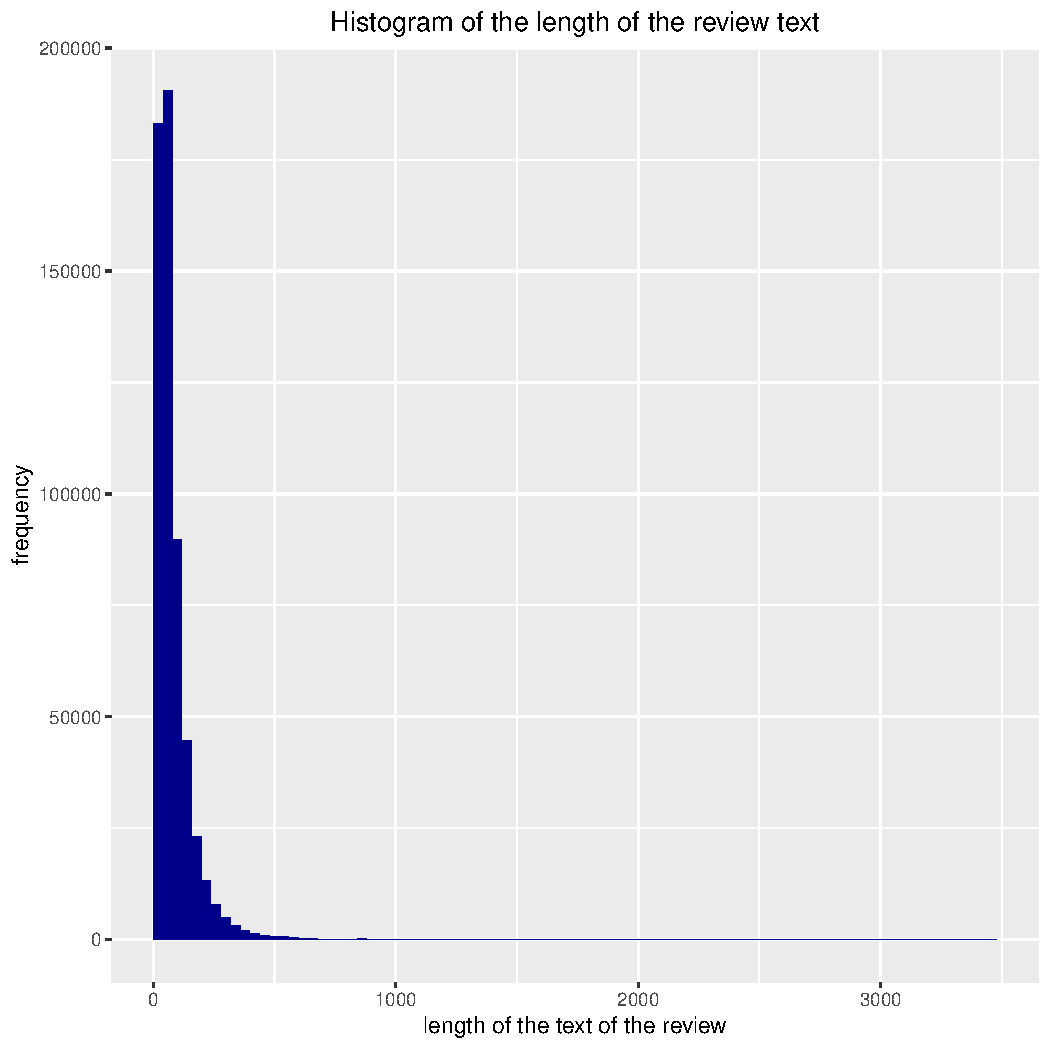
\includegraphics[width=0.9\columnwidth]{pics//plot_t_len.pdf} % Reduce the figure size so that it is slightly narrower than the column. Don't use precise values for figure width.This setup will avoid overfull boxes. 
\caption{Using the trim and clip commands produces fragile layers that can result in disasters (like this one from an actual paper) when the color space is corrected or the PDF combined with others for the final proceedings. Crop your figures properly in a graphics program -- not in LaTeX}
\label{fig1}
\end{figure}



\section{Data Analysis}

\subsection{Model}

\subsection{Empirical Evaluation}

\subsection{Discussion}


\section{References}

\bibliographystyle{aaai} \bibliography{bibfile1,bibfile2,...}


\end{document}
